\section{An analytic loss-limited EESM design map}
\label{sec:eesm-design-map}

The canonical coordinates of \cref{sec:whitening} give, without voltage,
\begin{equation}
 P_{\mathrm{Cu}}=z_\psi^2+z_q^2+z_0^2,
 \qquad M=\kappa z_\psi z_q.
\end{equation}
Because \(2|z_\psi z_q|\leq z_\psi^2+z_q^2\leq
P_{\mathrm{Cu},\max}\), equality requires
\(z_0=0\) and \(|z_\psi|=|z_q|=\sqrt{P_{\mathrm{Cu},\max}/2}\).
Therefore
\begin{equation}
 \boxed{M_{\max}^{(U\,\mathrm{free})}
 =\frac{\kappa}{2}P_{\mathrm{Cu},\max}.}
 \label{eq:eesm-mmax-loss}
\end{equation}
This is also the largest eigenvalue of the loss-whitened torque matrix times
the loss budget.

The coefficient follows from the original parameters, not from curve fitting.
With \(a=3R_s/2\) and \(b=R_{\mathrm{exc}}\), the active-flux coefficient in
whitened coordinates has norm
\begin{equation}
 \beta^2=\frac{\Delta L^2}{a}+\frac{L_{\mathrm{exc}}^2}{b}.
\end{equation}
Since the whitened quadrature current contributes another factor
\(1/\sqrt a\),
\begin{equation}
 \boxed{\kappa=k_T\sqrt{\frac{\Delta L^2}{a^2}
 +\frac{L_{\mathrm{exc}}^2}{ab}}.}
 \label{eq:kappa-machine-parameters}
\end{equation}
The two natural machine coordinates are consequently
\begin{equation}
 \gls{sym:xm}=\frac{\Delta L}{a},\qquad
 \gls{sym:ym}=\frac{L_{\mathrm{exc}}}{\sqrt{ab}},\qquad
 \gls{sym:rm}=\sqrt{x_M^2+y_M^2}.
 \label{eq:machine-coordinates}
\end{equation}
Both have units of seconds: henry per ohm is a time constant.  Calling them
dimensionless would be incorrect.  Their meaning is nevertheless direct.
The signed coordinate \(x_M\) measures reluctance-torque coupling per stator
loss price; \(y_M\) measures field-excitation coupling relative to the
geometric mean of stator and rotor loss prices.  Their radius satisfies
\begin{equation}
 \boxed{\frac{M_{\max}}{P_{\mathrm{Cu},\max}}
 =\frac{k_T}{2}r_M.}
 \label{eq:torque-per-loss-radius}
\end{equation}

For a dimensionless plot choose, and report, a positive reference frequency
\(\gls{sym:omegab}\).  Then
\begin{equation}
 \gls{sym:Xm}=\omega_bx_M,\qquad
 \gls{sym:Ym}=\omega_by_M,\qquad
 \gls{sym:cm}=\sqrt{X_M^2+Y_M^2}
 =\frac{2\omega_bM_{\max}}{k_TP_{\mathrm{Cu},\max}}.
 \label{eq:dimensionless-capability}
\end{equation}
Changing \(\omega_b\) changes only the numerical scale, not rankings or
angles.  A torque requirement becomes the exterior of a circle,
\begin{equation}
 \boxed{x_M^2+y_M^2\geq
 \left(\frac{2M_{\mathrm{req}}}{k_TP_{\mathrm{Cu},\max}}\right)^2.}
 \label{eq:machine-capability-circle}
\end{equation}
The mechanism angle
\(\gls{sym:phim}=\operatorname{atan2}(y_M,x_M)\) distinguishes equal-radius
machines.  Near the horizontal axis the capability is mainly reluctance
coupling; near the vertical axis it is mainly wound-field coupling.  A
negative \(\Delta L\) places a machine in the left half-plane, but does not
mean negative capability: the optimal \(i_d\) sign changes so that
\(\Delta L i_di_q\) is positive.  Hence quadrants encode sign convention and
optimal current orientation, not good and bad machine classes.

\begin{figure}[tb]
\centering
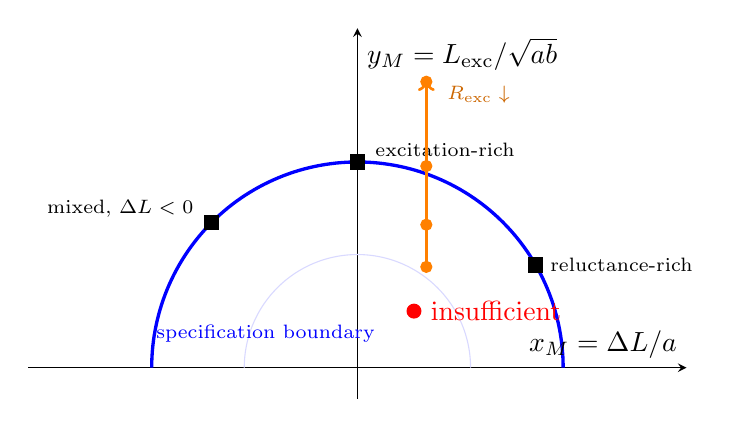
\begin{tikzpicture}
\begin{axis}[
 width=.82\linewidth,height=.55\linewidth,
 axis equal image,axis lines=middle,xmin=-3.2,xmax=3.2,ymin=-.3,ymax=3.3,
 xlabel={$x_M=\Delta L/a$},ylabel={$y_M=L_{\mathrm{exc}}/\sqrt{ab}$},
 ticks=none,clip=false]
 \addplot[domain=0:180,samples=121,blue,very thick]
   ({2*cos(x)},{2*sin(x)});
 \addplot[blue!15,domain=0:180,samples=121] ({1.1*cos(x)},{1.1*sin(x)});
 \addplot[only marks,mark=*,mark size=2.5pt,red] coordinates {(.55,.55)};
 \node[red,anchor=west] at (axis cs:.62,.55) {insufficient};
 \addplot[only marks,mark=square*,mark size=2.6pt,black]
   coordinates {(1.73,1) (0,2) (-1.42,1.41)};
 \node[anchor=west,font=\scriptsize] at (axis cs:1.78,1) {reluctance-rich};
 \node[anchor=west,font=\scriptsize] at (axis cs:.08,2.12) {excitation-rich};
 \node[anchor=east,font=\scriptsize] at (axis cs:-1.5,1.55) {mixed, $\Delta L<0$};
 \addplot[orange,very thick,->] coordinates {(.67,.98) (.67,1.39) (.67,1.96) (.67,2.78)};
 \addplot[only marks,orange,mark=*] coordinates {(.67,.98) (.67,1.39) (.67,1.96) (.67,2.78)};
 \node[orange!80!black,anchor=west,font=\scriptsize] at (axis cs:.78,2.65)
   {$R_{\mathrm{exc}}\downarrow$};
 \node[blue,anchor=south west,font=\scriptsize] at (axis cs:-2.05,.15)
   {specification boundary};
\end{axis}
\end{tikzpicture}
\caption{Loss-limited EESM capability map.  Constant torque per copper loss
forms circles.  Points on one circle have equal scalar capability but different
physical mechanisms.  The orange synthetic sweep shows the false divergence
created when excitation resistance is driven toward zero without adding a
replacement field constraint.}
\label{fig:machine-capability}
\end{figure}



\subsection{Numerical sweep as a diagnostic, not machine data}

For the synthetic normalized case of \cref{eq:toy-case},
\(a=0.6\), \(b=0.7\), \(\Delta L=0.4\), \(L_{\mathrm{exc}}=0.9\),
and \(k_T=3\).  It gives
\begin{equation}
 (x_M,y_M)=(0.6667,1.3887),\qquad
 r_M=1.5403,\qquad M_{\max}/P_{\max}=2.3104.
\end{equation}
Halving \(R_{\mathrm{exc}}\) multiplies only \(y_M\) by \(\sqrt2\); changing
saliency moves horizontally; changing \(L_{\mathrm{exc}}\) moves vertically;
changing \(R_s\) moves both coordinates, but with different powers.  The
trajectory in \cref{fig:machine-capability} therefore exposes exactly which
modeled cost is being relaxed.  As \(b\downarrow0\), \(y_M\to\infty\) and the
loss-only capability diverges.  This is the parameter-space signature of the
free direction found in \cref{sec:loss-degeneracy}, not a prediction of an
infinitely capable physical machine.
